\documentclass{article}
\usepackage{nips13submit_e,times}
\usepackage{hyperref}
\usepackage{url}
\usepackage{subcaption}       % \begin{subfigure}
\usepackage{graphicx}

\title{User Interface Parsing}
\author{
Calvin Loncaric\\
Department of Computer Science and Engineering\\
University of Washington\\
Seattle, WA\\
\texttt{loncaric@cs.washington.edu}\\
\url{https://homes.cs.washington.edu/\~loncaric}}
\date{June 8, 2015}

\newcommand{\fix}{\marginpar{FIX}}
\newcommand{\new}{\marginpar{NEW}}

\nipsfinalcopy % Uncomment for camera-ready version

% Useful tips:
%
%    \verb+text+      verbatim text
%
% \begin{table}[t]
% \caption{Sample table title}
% \label{sample-table}
% \begin{center}
% \begin{tabular}{ll}
% \multicolumn{1}{c}{\bf PART}  &\multicolumn{1}{c}{\bf DESCRIPTION}
% \\ \hline \\
% Dendrite         &Input terminal \\
% Axon             &Output terminal \\
% Soma             &Cell body (contains cell nucleus) \\
% \end{tabular}
% \end{center}
% \end{table}
%
% \begin{figure}[h]
% \begin{center}
% %\framebox[4.0in]{$\;$}
% \fbox{\rule[-.5cm]{0cm}{4cm} \rule[-.5cm]{4cm}{0cm}}
% \end{center}
% \caption{Sample figure caption.}
% \end{figure}

\begin{document}
\maketitle

\begin{abstract}
While easy to describe on paper, user interfaces are still tedious to construct
on a computer. Many programmer work hours are wasted translating design sketches
into code. There is a need for a tool which can automatically translate hand-%
drawn sketches into code without programmer assistance. In this work I describe
a possible approach to this problem using computer vision techniques. All code
and artifacts for this work are available online%
\footnote{\url{https://github.com/Calvin-L/ui-parser}}.
\end{abstract}

\section{Related Work}

The task of parsing a sketch of a user interface can be broken down into three
parts:
\begin{enumerate}
\item what UI elements are present? (e.g. text, images, forms, spacers)
\item what are the layout constraints? (e.g. widths, heights, paddings,
    containment relationships)
\item what is the simplest layout which contains all the elements and satisfies
    the given constraints?
\end{enumerate}

Thus, three bodies of work relate directly to this project: sketch recognition,
handwriting recognition, and constraint solvers.

Sketch recognition techniques have been developed for several domains, including
circuit diagrams and flowcharts. There have ben been efforts to simplify the
task, allowing experts to declaratively write descriptions of objects and have
the computer parse them from sketches \cite{ShapeDescriptions2004,
SketchREAD2007}.

While promising, these sketch recognition engines alone are not able to
effectively use context information (i.e. nearby drawing elements) to improve
accuracy. The approach I describe in \autoref{sec:element-detection} relies
almost exclusively on observations of surrounding elements in order to parse the
sketch.

Accurate handwriting recognition is needed in order to parse text and
annotations in user interface sketches. Handwriting recognition is an
extensively studied problem in computer vision \cite{HandwritingRecSurvey2000},
yet there do not seem to be any freely available off-the-shelf tools for finding
and recognizing sparse text on sketches.

In this work I used Google's Tesseract library \cite{Tesseract}, but Tesseract
is optimized for book text and the quality of the tool could be vastly improved
with a better handwriting recognition algorithm. More details are written in
\autoref{sec:constraint-formation}.

Microsoft's Z3 \cite{Z32008} is one of the most efficient and widely-used
constraint solvers. Z3 is a very general solver and can solve systems of
constraints involving booleans, integers, real numbers, arrays, and other
high-level types. Given the complex, hierarchical nature of user interfaces,
however, Z3 is a poor choice. There exist several constraint solvers
specifically for the domain of user interfaces; SkyBlue \cite{SkyBlue1994} is
one notable example. Researchers have also studied constraint-based layout
specifications for the web \cite{ConstraintsForTheWeb1997}.

In this work, I do not intend to solve the problem of layout generation from
constraints. The algorithm currently implemented in the tool uses a set of
handwritten heuristics (described in \autoref{sec:layout-gen}) and could
persumably be replaced with a smarter approach given more engineering time.

\section{Framework}

This section describes the actual operation of the tool. The input is a sketch
(such as one from \autoref{fig:sample-inputs}) and the output is a user
interface in the form of an HTML page (as in \autoref{fig:sample-outputs}).

\subsection{Element Detection}
\label{sec:element-detection}

The first major task for the tool is to identify the major \emph{elements} of
the sketch---that is, all the boxes, text, and measurement lines present. Text
is identified using the Tesseract library. For the remaining elements, the
algorithm proceeds in three minor stages: find line segments using the Hough
transform, vote on the explanation for each line segment, and then group line
segments into elements.

To find line segments, the tool first applies the probabilistic Hough transform
\cite{HoughTransform2000} to the image. This yields a series of partial line
segments which can be grouped into true line segments by merging parallel nearby
ones.

Each line segment then independently votes for what it believes itself to be and what it believes its relationship is to its neighbors. This is done using a few simple heuristics:
\begin{itemize}
\item a line that has a perpendicular line near each endpoint and a text box
    with a number nearby is a measurement line
\item a horizontal line with two perpendicular lines who have endpoints close to
    its endpoints is either a box top or a box bottom
\item box left sides and right sides are identified with a variant of the
    previous rule
\end{itemize}

With votes placed, a greedy algorithm then proceeds to find the best possible
box until no more boxes can be formed. The remaining lines are explained as
either noise or as constraint measurements, depending on whether a measurement
text box can be found for them.

\subsection{Constraint Formation}
\label{sec:constraint-formation}

The second task for the tool is to construct constraints for each element.
Constraints come in three major forms: containment constraints (i.e. element A
is contained within element B), size constraints (i.e. width and height) and
distance constraints (i.e. how far is it from one edge to another).

Containment constraints are generated using a simple box-intersection rule: if
one box is completely contained with another, then the latter contains the
former. Whether the one is a \emph{direct} child of the other or a
\emph{transitive} child of the other is determined later (see
\autoref{sec:layout-gen}).

Width and height constraints are identified by looking for constraint
measurements which relate two edges of the same box to each other. All remaining
constraints are treated as distance constraints.

The quality of the generated constraints is highly dependent on the quality of
the handwriting recognition which takes place at the beginning of the pipeline.
I found this to be a major bottleneck in the tool, and a good handwriting
recognizer is absolutely a requirement before this tool is usable.
Unfortunately, I did not have time to implement a good one (it might be an
entire research project on its own).

\subsection{Layout Generation}
\label{sec:layout-gen}

The final task for the tool is layout generation. At a high level, the layout
generation engine works by recursively identifying all the roots of the layout
(i.e. elements which are not constrained to be contained within another
element). Once the roots are found, the algorithm groups elements by which root
they belong to and recurses. Elements belonging to more than one root are
arbitrarily assigned to one.

For each root, the algorithm then finds a constraint for top, left, bottom, and
right margins; width; and height. Additional or conflicting constraints are
discarded. Any missing values are filled in by estimating distances from the
original sketch. The resulting values are written out as CSS. Random background
colors are chosen for each UI element to make reading the layout easier.

\section{Results and Discussion}

\begin{figure}[h]
\begin{center}
    \begin{subfigure}[b]{0.3\textwidth}
        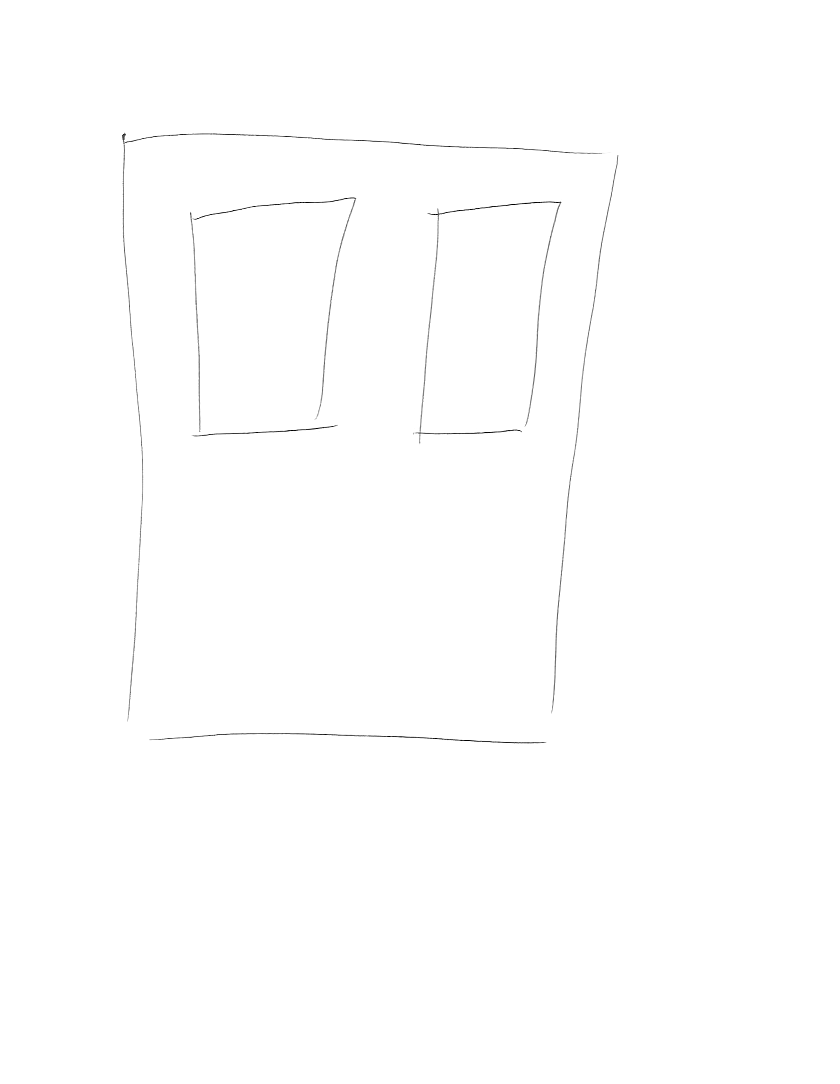
\includegraphics[width=\textwidth]{../examples/scan-01.png}
        \caption{\texttt{scan-01.png}}
    \end{subfigure}
    \begin{subfigure}[b]{0.3\textwidth}
        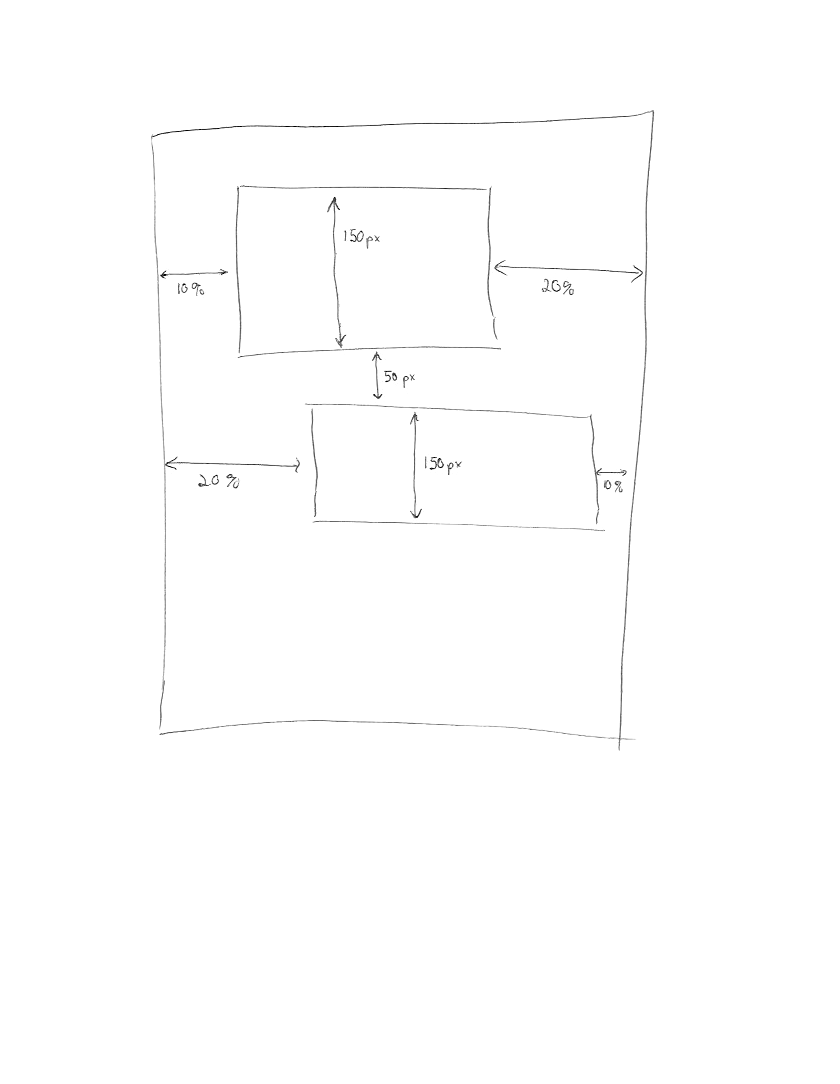
\includegraphics[width=\textwidth]{../examples/scan-04.png}
        \caption{\texttt{scan-04.png}}
    \end{subfigure}
    \begin{subfigure}[b]{0.3\textwidth}
        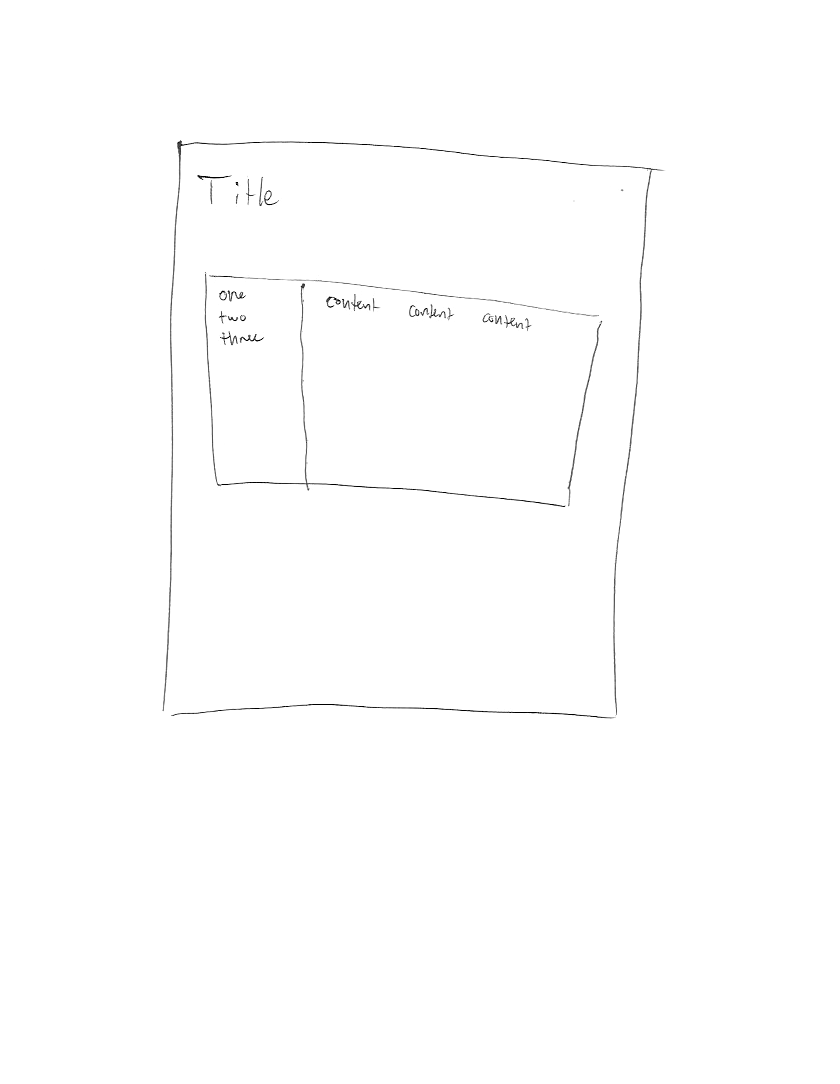
\includegraphics[width=\textwidth]{../examples/scan-08.png}
        \caption{\texttt{scan-08.png}}
    \end{subfigure}
\end{center}
\caption{A few sample inputs. The sketches ranged from simple (just boxes, no
    explicit constraints) to moderate (just boxes with explicit constraints) to
    complex (numerous UI elements including text, images, and tables).}
\label{fig:sample-inputs}
\end{figure}

\begin{figure}[h]
\begin{center}
    \begin{subfigure}[b]{0.3\textwidth}
        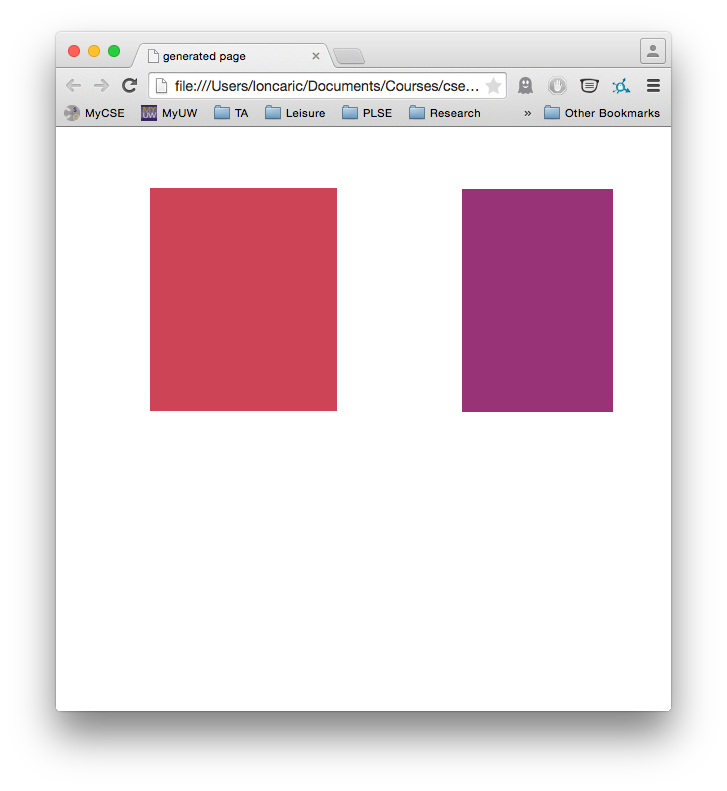
\includegraphics[width=\textwidth]{scan-01-output.png}
        \caption{\texttt{scan-01.png}}
    \end{subfigure}
    \begin{subfigure}[b]{0.3\textwidth}
        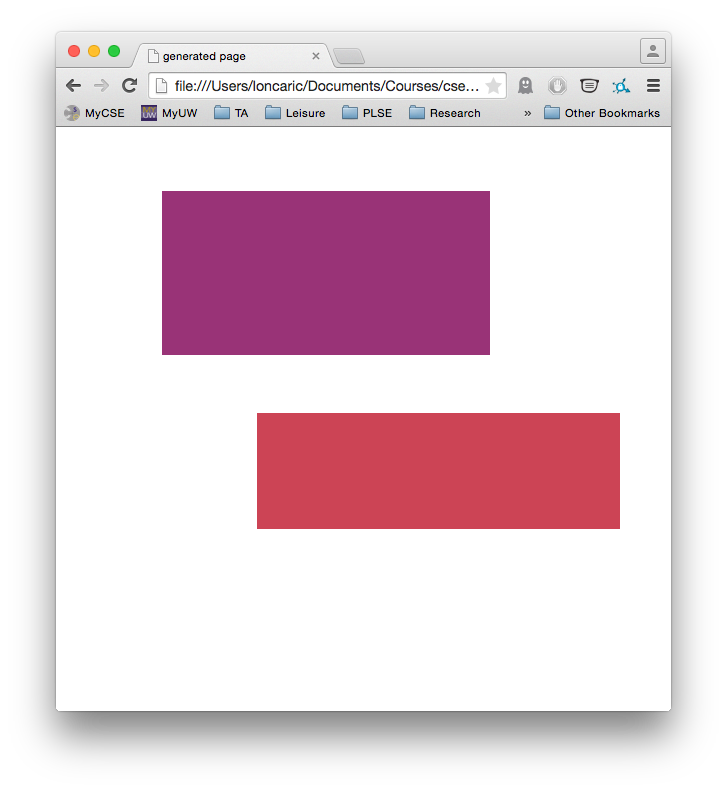
\includegraphics[width=\textwidth]{scan-04-output.png}
        \caption{\texttt{scan-04.png}}
    \end{subfigure}
    \begin{subfigure}[b]{0.3\textwidth}
        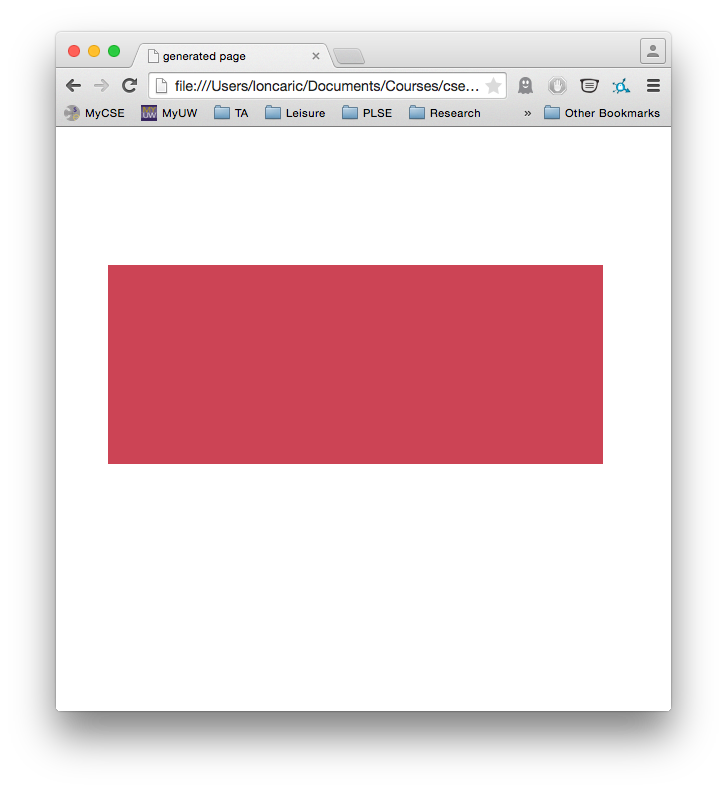
\includegraphics[width=\textwidth]{scan-08-output.png}
        \caption{\texttt{scan-08.png}}
    \end{subfigure}
\end{center}
\caption{Output screenshots for the sample images in
\autoref{fig:sample-inputs}.}
\label{fig:sample-outputs}
\end{figure}

\begin{table}[h]
\begin{center}
\input{benchmark.tex}
\end{center}
\caption{Timings and output qualities for each of the example inputs. The
    timings were collected on a 2012 MacBook Pro with a 2-core 2.5 GHz Intel
    Core i5 processor and 8 Gb of RAM. The output quality is a qualitative
    measure manually assessed by the author for each file. ``Perfect'' means
    that the output layout perfectly matched the input sketch. ``Good'' means
    that all major layout elements were identified, but some measurements were
    off. ``Bad'' means that some layout elements were missing and/or many
    measurements were off. ``Fail'' means that the output did not resemble the
    input sketch.}
\label{tbl:benchmarks}
\end{table}

At the beginning of the project I drew and scanned 13 sample layouts. Results
for each one are summarized in \autoref{tbl:benchmarks}. To give some indication
of what these sample inputs look like, a few selected images are shown in
\autoref{fig:sample-inputs}, with corresponding outputs in
\autoref{fig:sample-outputs}.

While the tool performs very well on early examples involving only boxes and
constraints, I did not have time to complete the project and implement parsing
for more complex elements (e.g. text, images, or tables). The presence of more
complex elements is what causes scores of ``bad'' and ``fail'' on many inputs.
As a general rule, the tool performs perfectly on inputs with just boxes (it
guesses at constraints fairly well), but due to limitations in the handwriting
recognition code it cannot reliably understand constraints, earning a score of
merely ``good'' on many examples.

\section{Conclusion}

While the user interface parser is far less capable than the ambitious goals set
out for it, it still does an adequate job on very simple layout files. A few
eningeering improvements could make it a very capable tool indeed.

As future research work, I would suggest investigating the problem of
handwriting recognition. For this tool we need a library which can reliably find
sparse text on a page and identify it. Existing off-the-shelf solutions seem
insufficient. Commercial solutions exist, but the research and development
community could surely benefit from an openly available toolset.

The most difficult part of this project was to optimize the very deep pipeline I
implemented. Even if each step in the tool is 99 percent accurate, the overall
pipeline still has very low quality. Each step has to be able to handle
imperfections from its predecessors.

The most important technique I used which improved recognition quality was the
independent voting step described in \autoref{sec:element-detection}. This had
two primary benefits. First, it is very robust to error: even if one line makes
an incorrect vote, its neighbors will typically place correct votes on its
behalf. Second, it gives a clear objective function to the next pipeline step:
explain as many votes as possible. The votes do not come with an associated
confidence, but I predict that adding one might improve quality even further.

\bibliography{bibliography}{}
\bibliographystyle{unsrt}

\end{document}
